%Copyright (C) 2014 Sergio García Villalonga.

A l'hora de realitzar les proves de localització, l'AirPlace Tracker proporciona dos modes: l'on-line i l'off-line. El primer mostra la posició estimada de l'usuari en cada moment. Es tracta d'un sistema molt visual però que no aporta cap tipus de dada que pugui ser analitzada posteriorment.

El mode off-line, per contra, pren un fitxer amb informació sobre diferents localitzacions i la potència del senyal rebut en cada una d'elles. Tècnicament, aquest fitxer es genera de la mateixa manera que el mapa de ràdio inicial, encara que, per evitar confusió, se l'anomenarà mapa de proves.

A partir del mapa de ràdio i de la informació sobre la intensitat del senyal a cada punt del mapa de proves, l'AirPlace Tracker estima la posició de les localitzacions del darrer. L'AirPlace tracker permet dur a terme aquest procés d'estimació amb diferents algorismes.

Aquest procés sí genera una sèrie de dades que poden ser analitzades estadísticament a posteriori. Per tal d'estudiar la influència del nombre d'usuaris en la precisió de la localització s'han generat dos mapes de proves, amb idèntiques localitzacions però preses en dos moments on la diferència d'usuaris fos significativa.

A continuació s'exposen els detalls de la presa de dades i els resultats obtinguts del seu anàlisi.

\subsection{Presa de dades}

La presa de dades per realitzar un anàlisi "off-line" de localitzacions en interior amb l'AirPlace Tracker comença amb la creació d'un mapa de prova utilitzant l'AirPlace Logger. Per aquest estudi en concret, se n'han creat dos, a exactament la mateixes localitzacions però en diferents contexts, un en absència d'altres usuaris i un altre en la situació contrària.

La recollida de dades amb una presència mínima a l'entorn (figura \ref{fig:foto_buit}) es va dur a terme en un context similar a la de la creació del mapa de ràdio: a partir de les 8 del matí pels passadissos i a partir de les 10 dins les botigues. Pel segon mapa de proves, les dades es varen recol·lectar els dies 20 i 21 de desembre de 2014 a la tarda. Com s'aprecia a la figura \ref{fig:foto_ple}, en el segon l'ocupació del centre és major.

\begin{figure}[ht]
\begin{center}
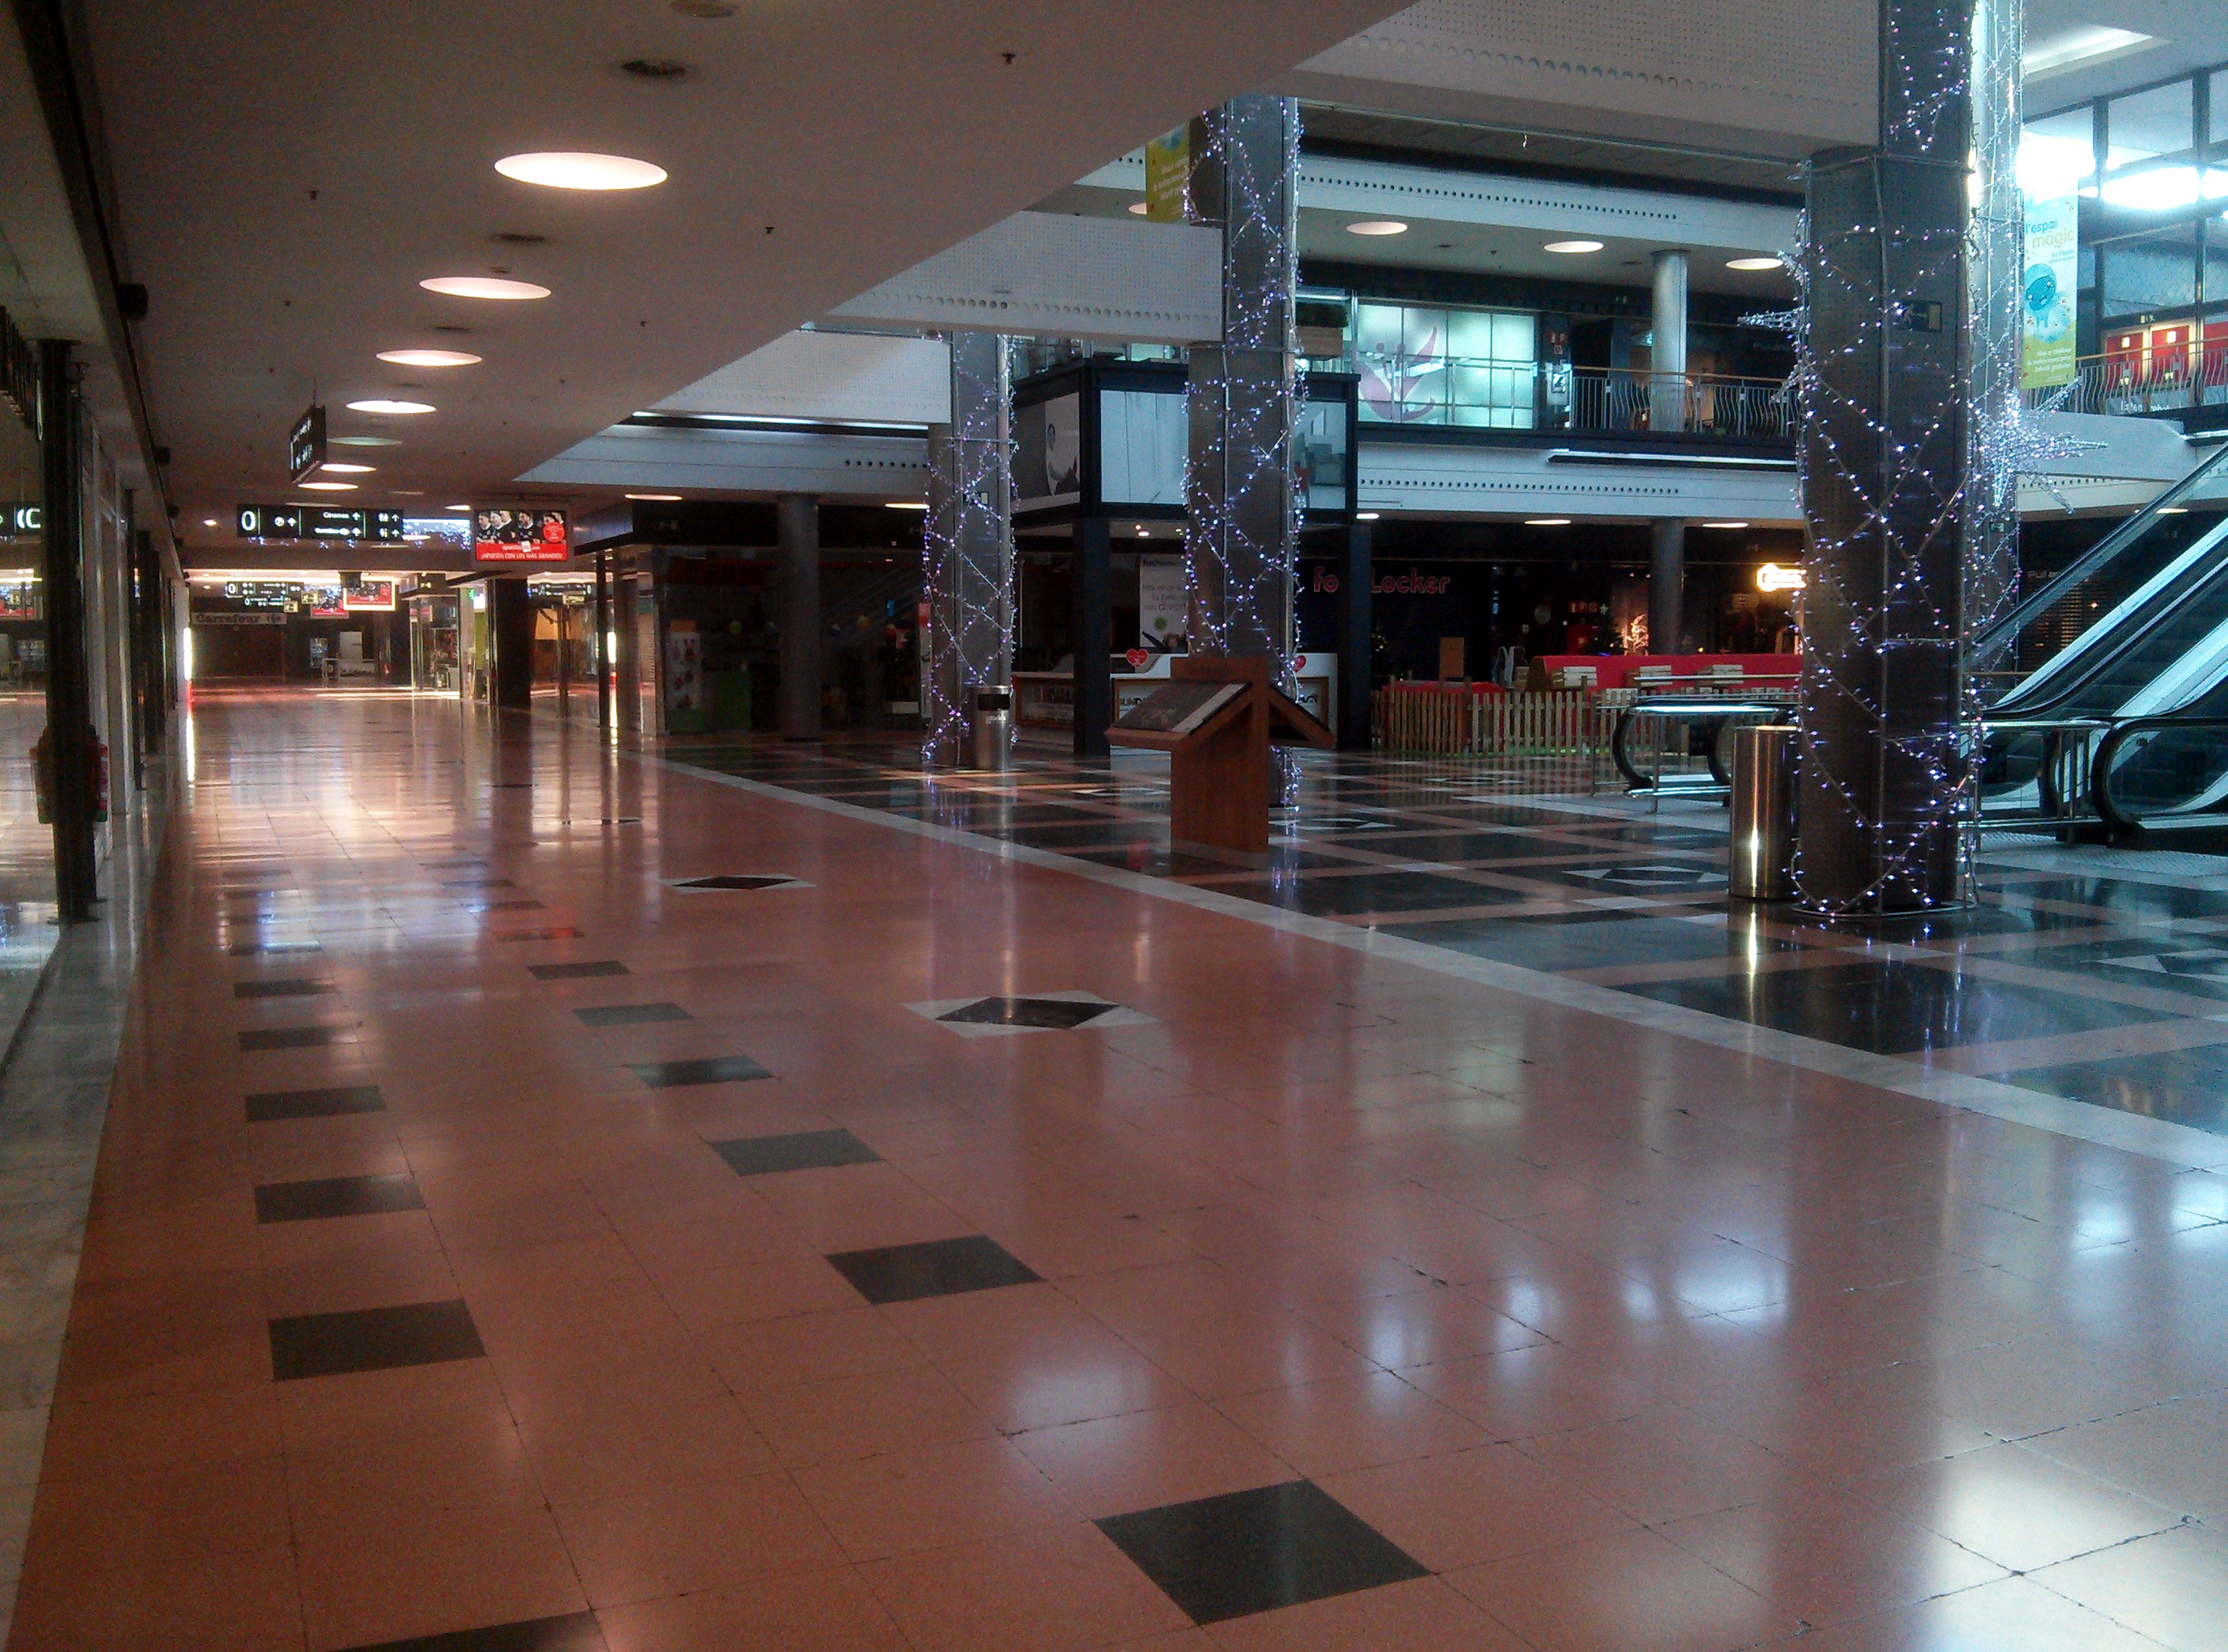
\includegraphics[width=7cm]{imatges/foto_buit.jpg}
\caption{Centre comercial en les proves sense usuaris.}
\label{fig:foto_buit}
\end{center}
\end{figure}

\begin{figure}[ht]
\begin{center}
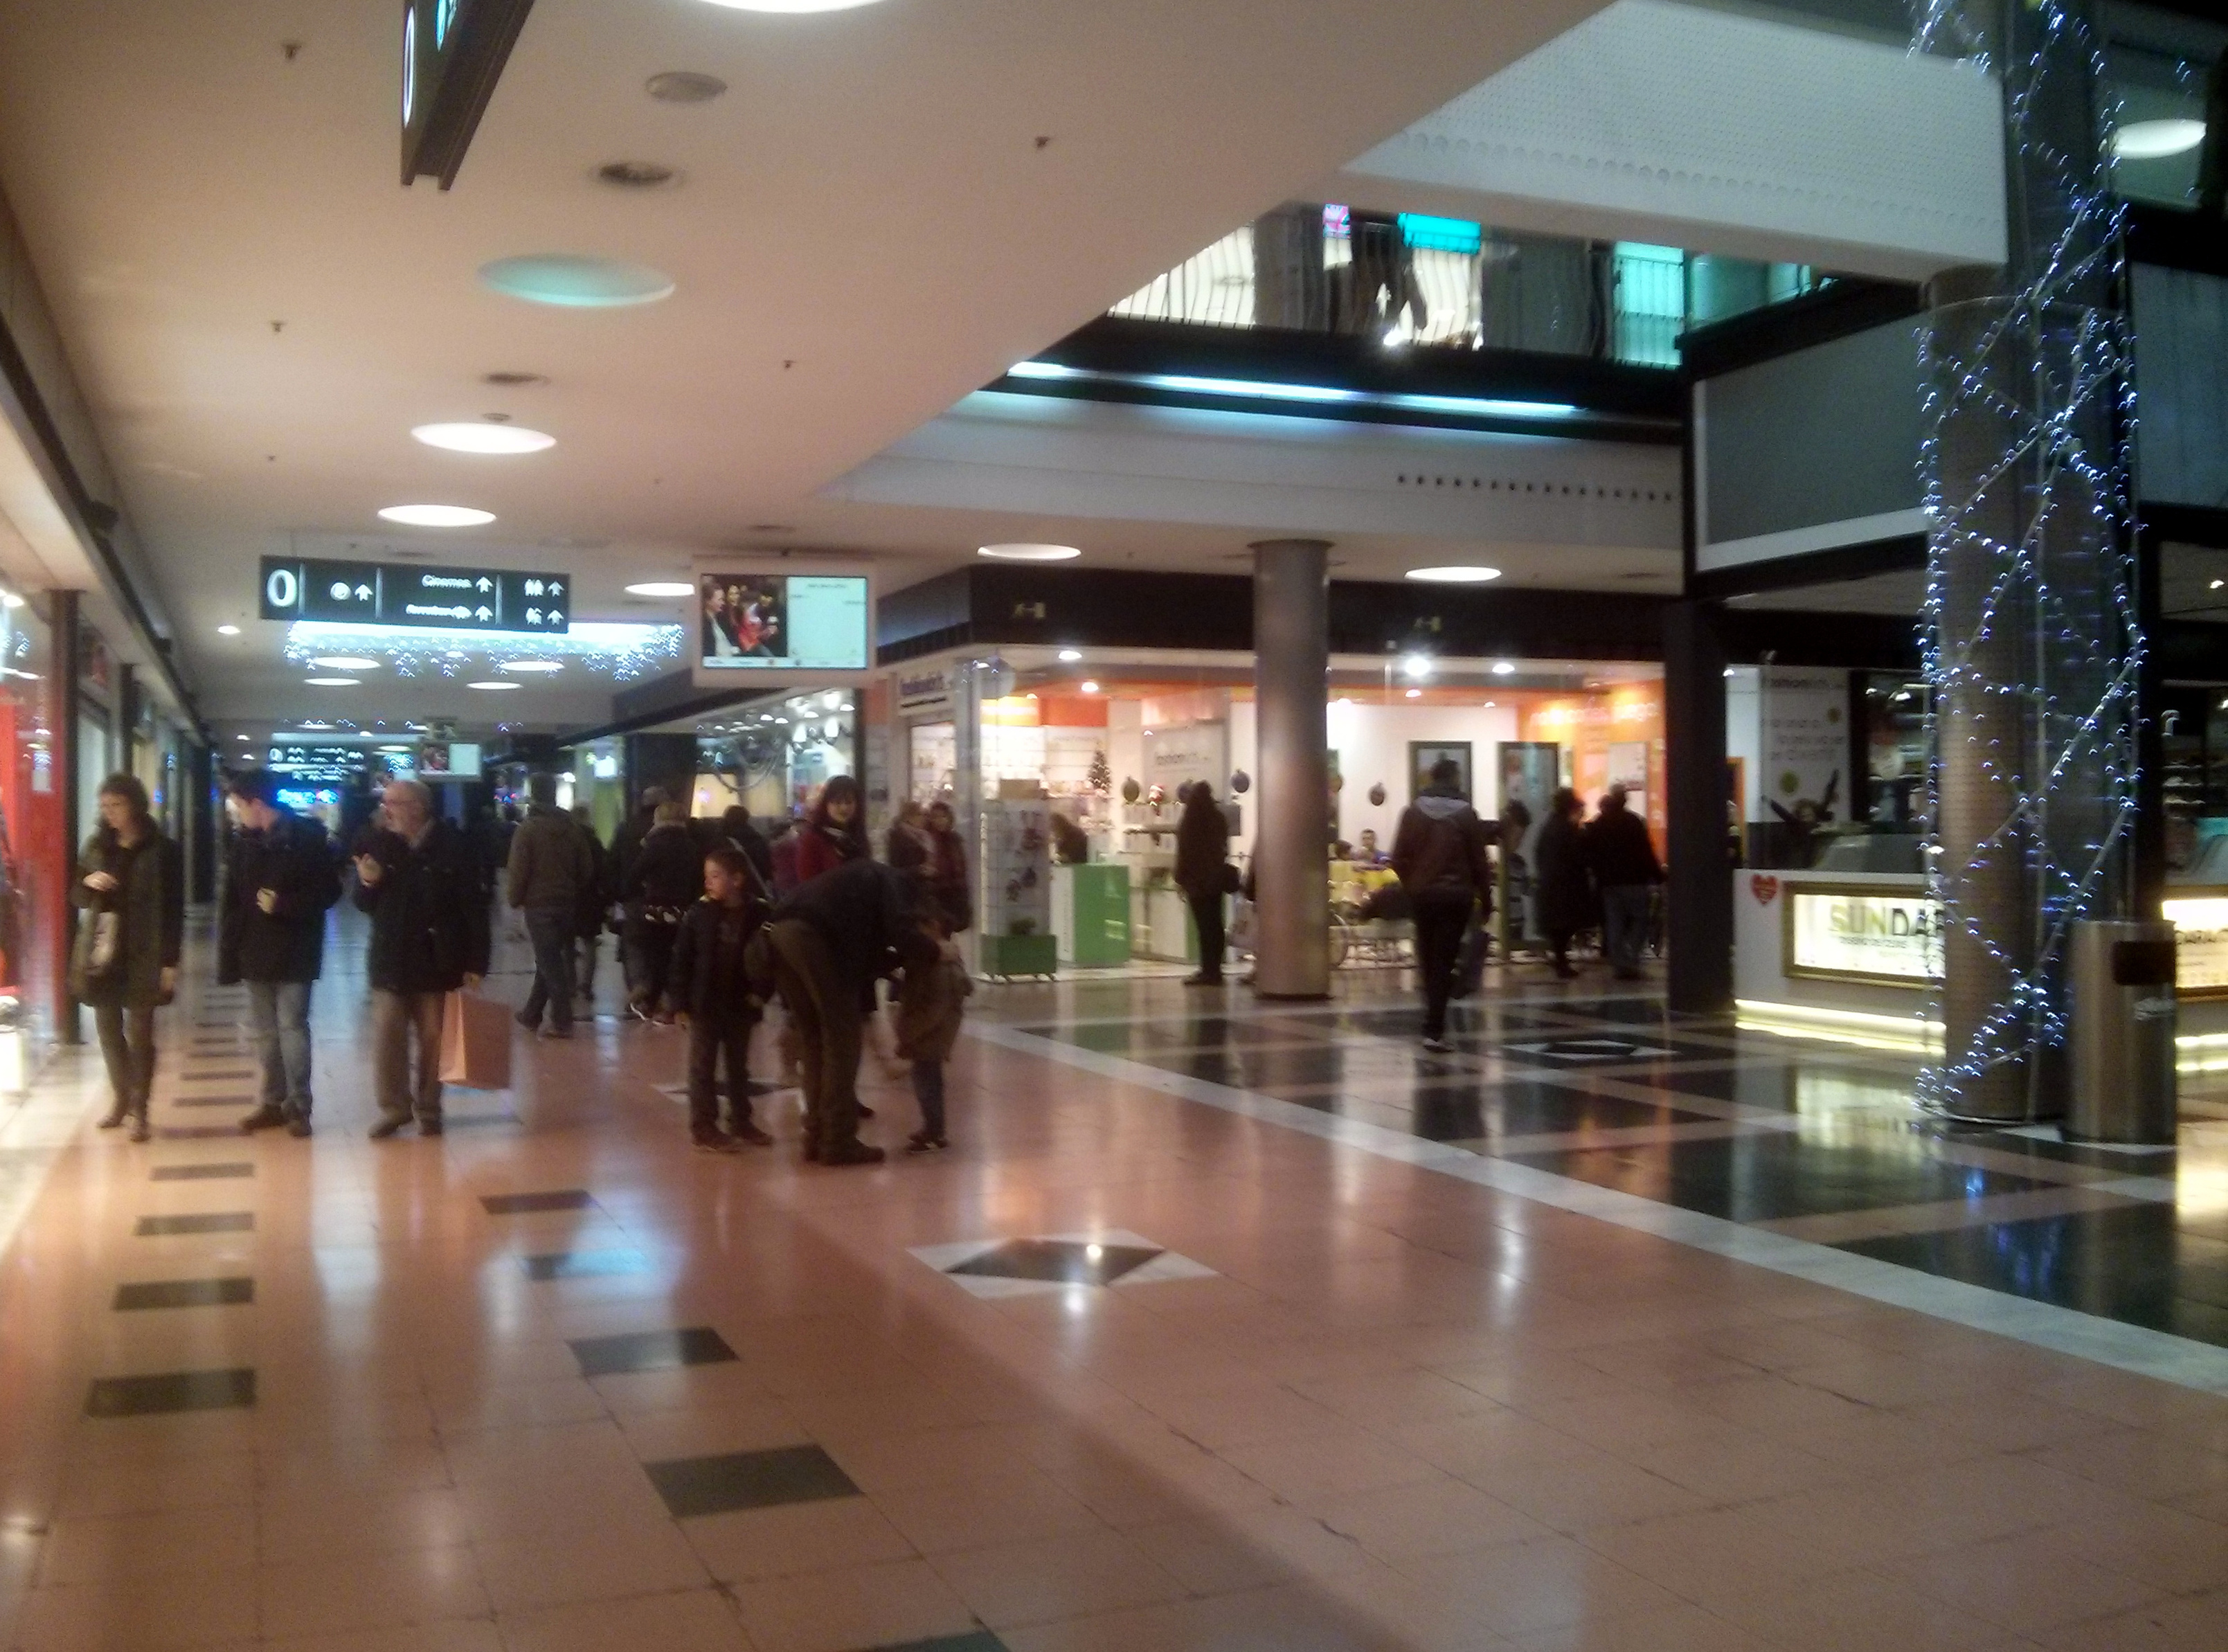
\includegraphics[width=7cm]{imatges/foto_ple.jpg}
\caption{Centre comercial en les proves en horari comercial.}
\label{fig:foto_ple}
\end{center}
\end{figure}

En ambdós contexts, s'han pres mostres a 115 diferents posicions, (figura \ref{fig:planol_proves}), de les quals 42 es troben dins botigues i 73 a passadissos. A l'igual que en la creació del mapa de ràdio, per cada posició s'han pres 30 mostres. La distància mínima mitjana entre localitzacions és de 5,56 m.

\begin{figure}[ht]
\begin{center}
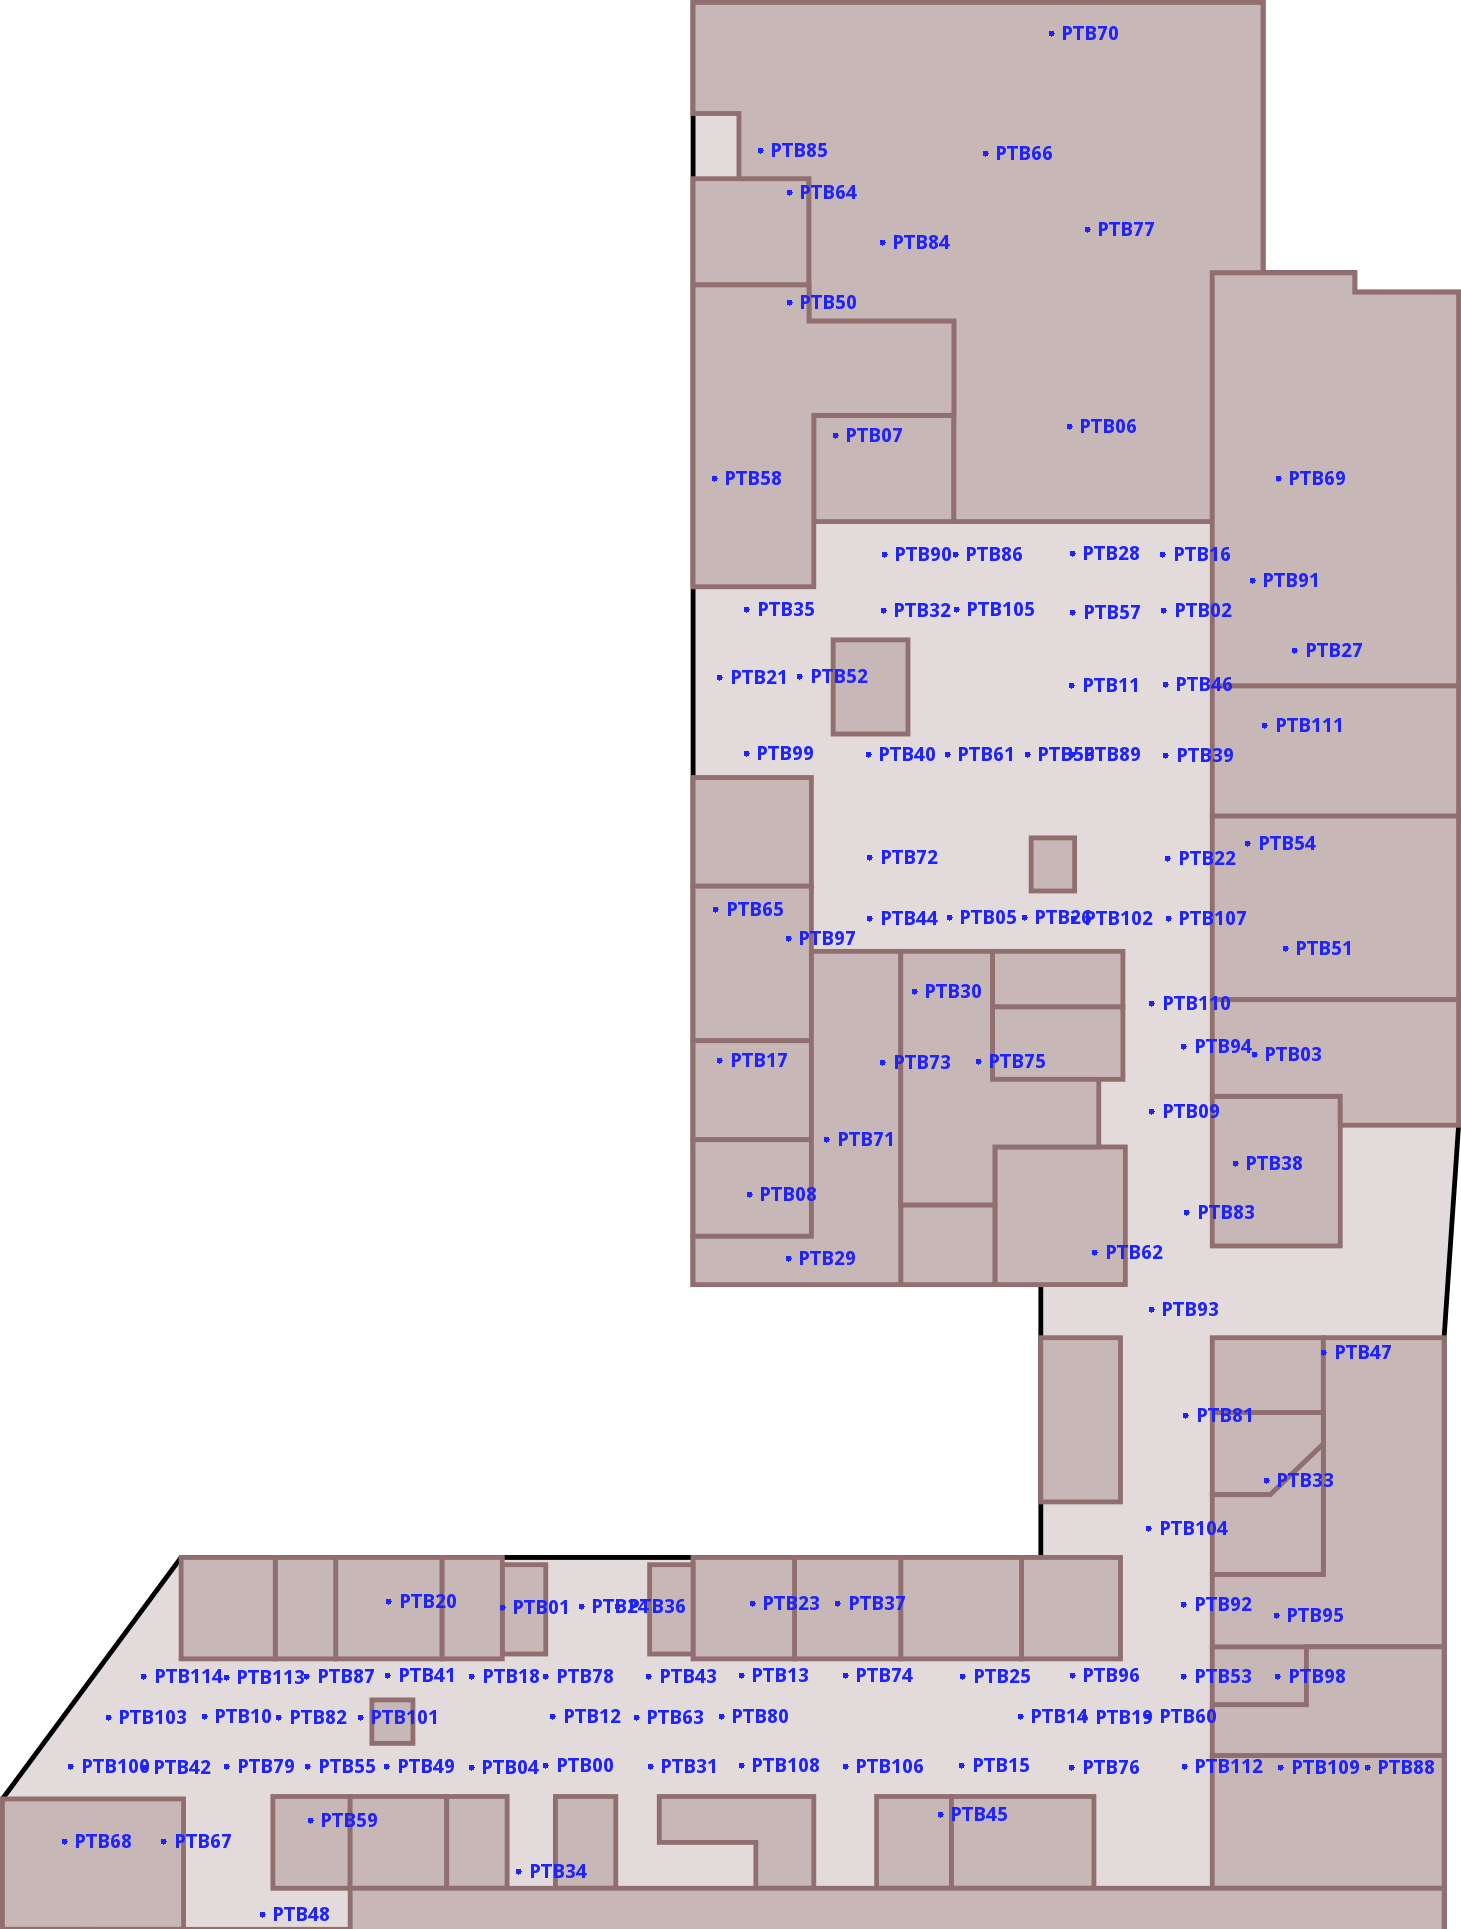
\includegraphics[width=7cm]{imatges/planol_proves.png}
\caption{Punts on s'ha dut a terme la presa de dades en les proves.}
\label{fig:planol_proves}
\end{center}
\end{figure}

\subsection{Estimació de les localitzacions de prova}

Per tal de realitzar un anàlisi detallat de les dades generades amb el mode "off-line" es proporcionen a l'AirPlace Tracker els mapes de prova generats anteriorment. Utilitzant el mapa de ràdio generat inicialment realitza les estimacions de cada una de les posicions de prova, tenint en compte la intensitat del senyal a cada una. Aquesta operació es pot realitzar repetidament i amb diferents algorismes, pel que ens permet estudiar de manera més detallada la influència d'usuaris a l'entorn.

De totes formes, el funcionament del mode "off-line" només proporciona, al final de l'execució de les estimacions, l'error mitjà de les posicions calculades respecte a les posicions reals del mapa de prova. Aquesta informació és mostrada en forma de finestra de diàleg en la mateixa aplicació (figura \ref{fig:analisi_offline_defecte}).

\begin{figure}[ht]
\begin{center}
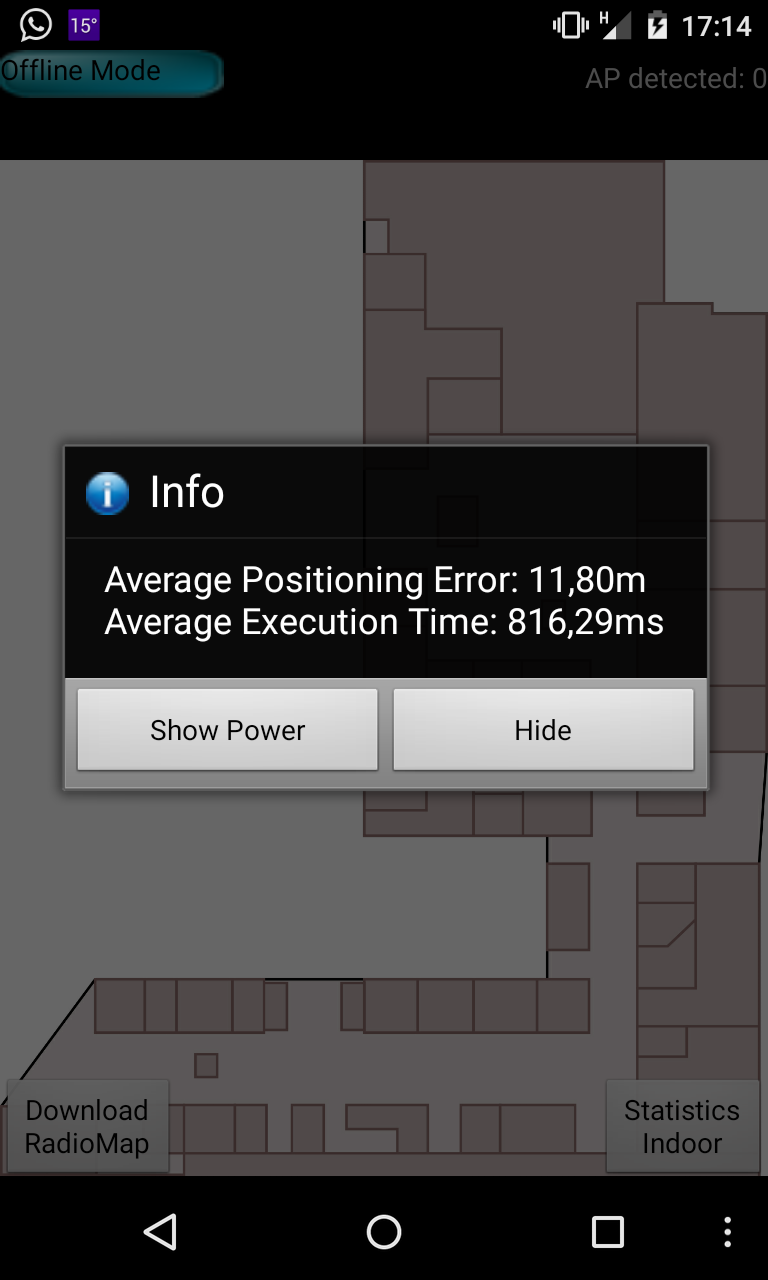
\includegraphics[width=5cm]{imatges/analisi_offline_defecte.png}
\caption{Final de l'execució d'un anàlisi off-line d'AirTracker.}
\label{fig:analisi_offline_defecte}
\end{center}
\end{figure}

Un altre problema és el temps d'execució de les proves. Depenent de l'algorisme triat i dels paràmetres corresponents, l'anàlisi de l'error mitjà de les estimacions per una quantitat de localitzacions relativament gran porta, aproximadament, una mitja de 80 minuts. Aquest factor dificulta la realització d'anàlisis per diferents algorismes i paràmetres.

Per tal de generar resultats més detallats i poder dur a terme un anàlisi estadístic més ric, així com per agilitzar l'execució de les proves, es va decidir realitzar una sèrie de modificacions al codi de l'AirPlace Tracker \footnote{El codi modificat es pot trobar a \url{https://github.com/SeGarVi/TFM/tree/master/AirplaceTracker}}, aprofitant la seva llicència lliure. Amb aquestes modificacions, l'AirPlace Tracker executa en paral·lel els anàlisis amb diferents algorismes i persisteix els resultats dels anàlisis en forma de fitxers.

D'aquesta manera, els fitxers resultants de l'execució de l'anàlisi contenen informació sobre la posició real de cada localització de prova, la posició estimada, i l'error. Pel que fa a la paral·lelització, al tractar-se d'un telèfon amb un processador multinucli, permet l'execució de l'anàlisi amb els quatre algorismes disponibles (figura \ref{fig:analisi_offline_paralel}), simultàniament, en uns 110 minuts de mitjana.

\begin{figure}[ht]
\begin{center}
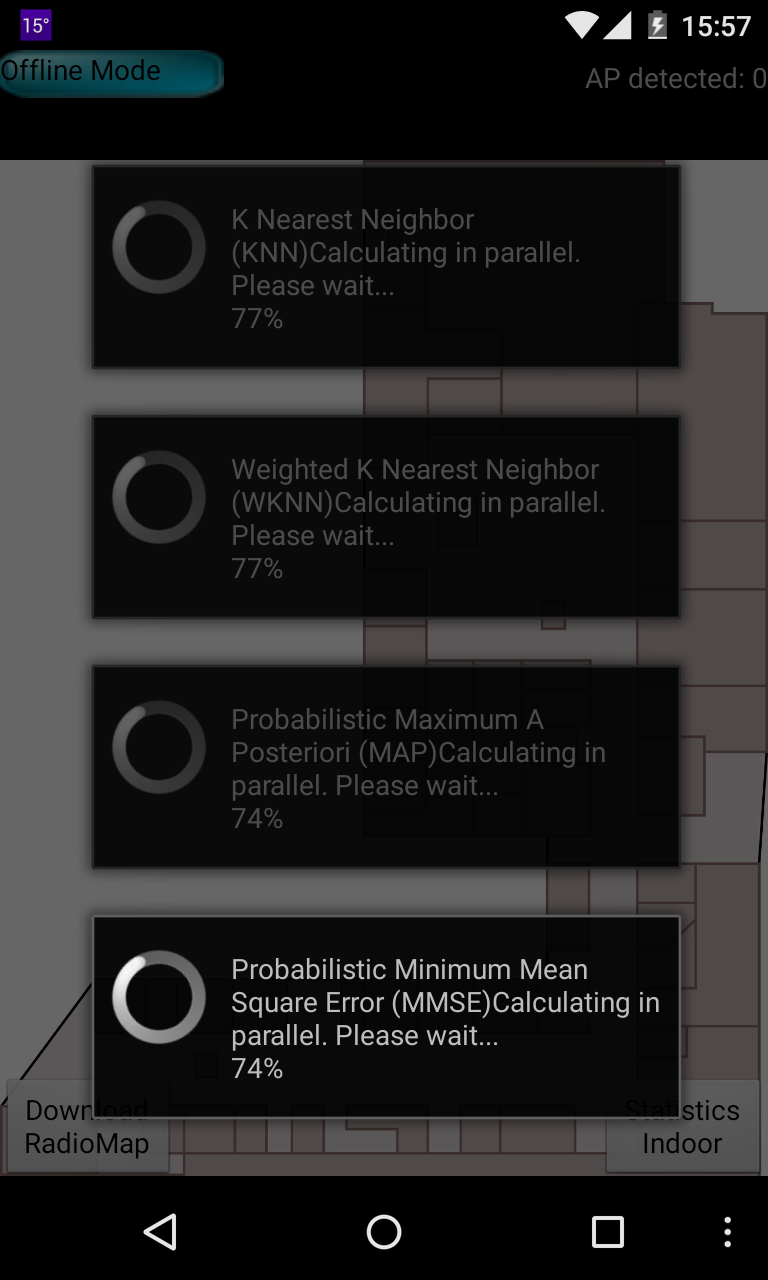
\includegraphics[width=5cm]{imatges/analisi_offline_paralel.png}
\caption{Execució d'un anàlisi en paral·lel amb AirTracker.}
\label{fig:analisi_offline_paralel}
\end{center}
\end{figure}

\subsection{Anàlisi dels resultats}

El resultat obtingut en el processament dels mapes de proves permet obtenir l'error en el càlcul de la posició de cada localització. Aquestes dades, extretes dels mapes de prova realitzats  tant amb altres usuaris al voltant com sense, són la base per l'estudi de la influència d'aquests en la precisió del sistema.

De les 30 mostres enregistrades per cada localització als mapes de prova, s'ha decidit calcular l'error mitjà respecte a la posició real i la desviació mitjana de cada mostra. D'aquesta manera podem estudiar com afecta la presència d'usuaris tant a la precisió mitjana com a la dispersió de les estimacions. Els resultats de la comparativa s'han classificat per algorismes utilitzats, per situació de les localitzacions (passadís o botiga) i per context (amb presència i sense presència d'altres usuaris).

%La primera deducció a la que arribam amb l'anàlisi dels resultats anteriors és que mostra un %clar augment de l'error entre les estmacions en un entorn buit i un amb una quantitat considerable de persones. De totes maneres, es poden observar diferències notables depenent de l'algorisme, els paràmetres i si la posició és a un passadís o dins una botiga.

A continuació es comenten els resultats obtinguts classificats per algorisme.

\subsection{\textit{K Nearest Neighbors}}

L'algorisme de K Nearest Neighbors estima la posició en dues fases:

\begin{enumerate}
    \item Calcula la distància de la localització a estimar amb cada una de les localitzacions del mapa de ràdio basant-se en les dades d'intensitat del senyal de ràdio.
    \item Estima la posició calculant la mitja de les K localitzacions del mapa de ràdio més properes.
\end{enumerate}

Com es pot observar al gràfic (figura \ref{fig:grafic_mitja_KNN}), en el cas de les localitzacions dins botigues, la precisió mitjana en l'entorn sense usuaris és major que en el cas d'un entorn amb clients al voltant. En el cas dels passadissos, la mesura sense usuaris es més precisa fins K=8, a on passa a ser-hi menys, encara que sense gran diferència.

Les mesures més precises donen un error mitjà de 8,68 m., en l'entorn sense usuaris, i 9,82 en l'entorn contrari.

\begin{figure}[ht]
\begin{center}
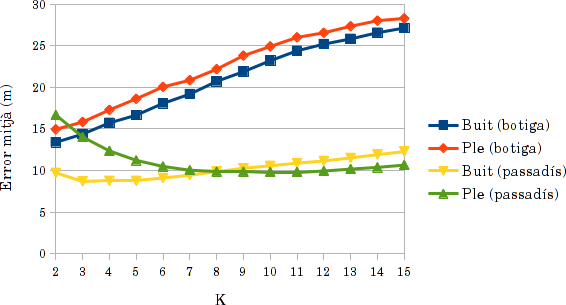
\includegraphics[width=7cm]{imatges/knn_mitja.png}
\caption{Comparació gràfica de l'error per l'algorisme \textit{K Nearest Neighbors} en passadissos (dalt) i botigues (abaix).}
\label{fig:grafic_mitja_KNN}
\end{center}
\end{figure}

Pel que fa a la desviació mitjana (figura \ref{fig:grafic_desviacio_KNN}) podem observar que tant dins botigues com en passadissos, la presència d'usuaris afecta negativament a la dispersió de les estimacions.

\begin{figure}[ht]
\begin{center}
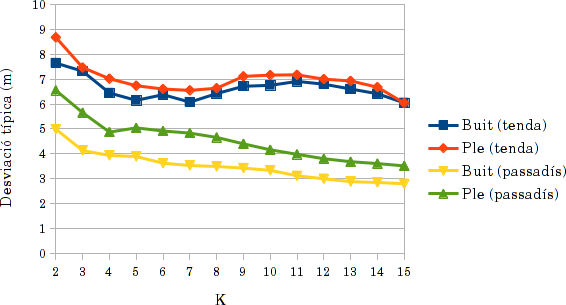
\includegraphics[width=7cm]{imatges/knn_desviacio.png}
\caption{Comparació gràfica de l'error per l'algorisme \textit{K Nearest Neighbors} en passadissos (dalt) i botigues (abaix).}
\label{fig:grafic_desviacio_KNN}
\end{center}
\end{figure}

\subsection{\textit{Weighted K Nearest Neighbors}}

L'algorisme Weighted K Nearest Neighbors segueix el mateix funcionament que l'anterior, només que a l'hora de calcular el punt mitjà de les K localitzacions més properes. La variable utilitzada per ponderar la mitja és la inversa de la distància. Per tant, a l'hora de realitzar la mitjana els punts de referència més propers tenen més pes que els llunyans, al suposar-se que les mesures de potència del senyal dels primers seran més precises.

En el cas de les proves amb l'algorisme \textit{Weighted K Nearest Neighbors}, la tendència és molt similar. Els gràfics (figura \ref{fig:grafic_mitja_WKNN}) mostren clarament com es segueix el mateix patró que amb l'anterior algorisme (figura \ref{fig:grafic_KNN}), encara que amb un error mitjà lleugerament menor.

Les mesures més exactes donen un error de 8,61 m, en un entorn sense altres usuaris i un error de 9,68 en l'entorn amb molta presència de clients.

\begin{figure}[ht]
\begin{center}
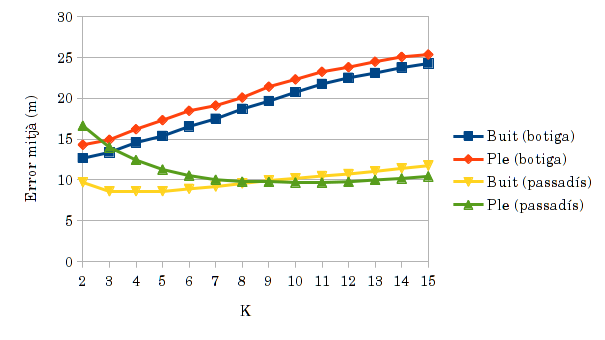
\includegraphics[width=7cm]{imatges/wknn_mitja.png}
\caption{Comparació gràfica de l'error per l'algorisme \textit{Weighted K Nearest Neighbors} en passadissos (dalt) i botigues (abaix).}
\label{fig:grafic_mitja_WKNN}
\end{center}
\end{figure}

En el cas de la dispersió de les estimacions (figura \ref{fig:grafic_desviacio_WKNN}), amb aquest algorisme observam el mateix comportament. En tots els casos, tant a passadissos com dins botigues, la dispersió en l'entorn amb altres usuaris present és major. 

\begin{figure}[ht]
\begin{center}
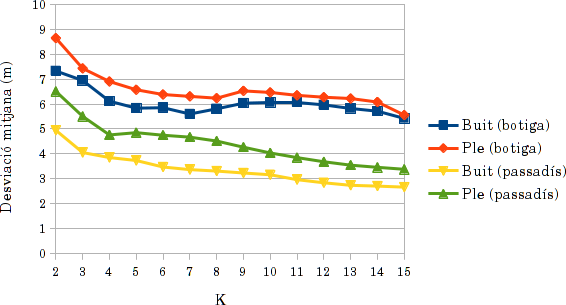
\includegraphics[width=7cm]{imatges/wknn_desviacio.png}
\caption{Comparació gràfica de l'error per l'algorisme \textit{Weighted K Nearest Neighbors} en passadissos (dalt) i botigues (abaix).}
\label{fig:grafic_desviacio_WKNN}
\end{center}
\end{figure}

\subsection{\textit{Probabilistic Maximum A Posteriori}}

Aquest algorisme estima la posició actual de l'usuari com el punt del mapa de ràdio que maximitza la probabilitat a partir de les dades d'intensitat del senyal. Per l'estimació de la probabilitat es fa servir la tècnica del mínim error quadràtic mitjà i el valor és ponderat amb una variable K, que penalitza inversament la probabilitat. D'aquesta manera, un valor baix de K dona com a resultat probabilitats molt similars entre la localització de l'usuari i els punts del mapa de ràdio, fet que pot derivar en que no es pugui estimar la localització.

Realitzant el càlcul amb l'algorisme \textit{Probabilistic Maximum A Posteriori} s'obté un patró diferent als anteriors. Com es pot observar, els valors de l'error mitjà minven conforme augmenta K en tots els casos (figura \ref{fig:grafic_mitja_MAP}). De totes maneres, la precisió no millora constantment, sinó que a partir de certs valors de K (K=8 a passadissos i K=7 en botigues) el valor d'error esdevé constant. De totes maneres, l'error mitjà de localització es veu afectat per la presència de clients tant dins botigues com en passadissos.

Pel que fa als millors registres de precisió, es troben en 11,35 m. en un entorn sense usuaris i 12,77 m. en el cas contrari.

\begin{figure}[ht]
\begin{center}
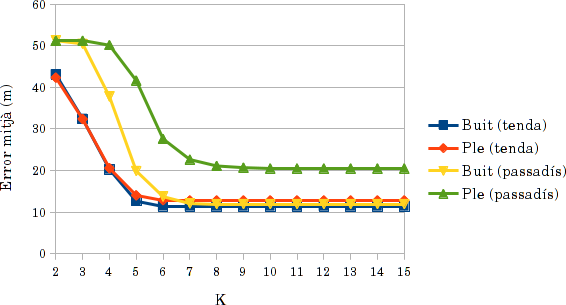
\includegraphics[width=7cm]{imatges/map_mitja.png}
\caption{Comparació gràfica de l'error per l'algorisme \textit{Probabilistic Maximum A Posteriori} en passadissos (dalt) i botigues (abaix).}
\label{fig:grafic_mitja_MAP}
\end{center}
\end{figure}

Pel que fa a la desviació mitjana de les estimacions \ref{fig:grafic_desviacio_MAP}), a partir de valors de K majors que 4, també es veu perjudicada per la presència d'altres usuaris, tant en botigues com en passadissos. A més, a l'igual que la mitjana, el seu valor s'estabilitza a partir de K=10.

\begin{figure}[ht]
\begin{center}
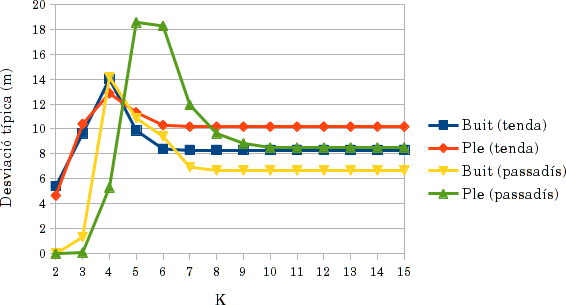
\includegraphics[width=7cm]{imatges/map_desviacio.png}
\caption{Comparació gràfica de l'error per l'algorisme \textit{Probabilistic Maximum A Posteriori} en passadissos (dalt) i botigues (abaix).}
\label{fig:grafic_desviacio_MAP}
\end{center}
\end{figure}

\subsection{\textit{Probabilistic Minimum Mean Square Error}}

En l'algorisme \textit{Probabilistic Minimum Mean Square Error} es duu a terme una estimació en dos passos:

\begin{enumerate}
    \item alcula la probabilitat de que l'usuari es trobi en cada un dels punts del mapa de ràdio de la mateixa manera que en l'algorisme anterior.
    \item Es calcula la posició de l'usuari com la mitjana ponderada dels punts del mapa de ràdio, utilitzant la probabilitat de que l'usuari es trobi a un punt com a variable de ponderació.
\end{enumerate}

Aquest algoritme, per tant, també es veu afectat per la variable K, de manera que a l'hora de calcular la mitjana ponderada, els punts amb més probabilitat tenen més pes.

En aquest darrer cas, l'anàlisi mostra un comportament similar a l'anterior però amb particularitats. A l'igual que amb l'algorisme \textit{Probabilistic Maximum A Posteriori}, a partir de cert valor de K (K=6 en passadissos i K=5 dins botigues), l'error mitjà s'estabilitza. Aquesta estabilització es deu a que els valors alts de K afavoreixen les estimacions amb més probabilitat.

La principal diferència s'observa en el comportament amb valors petits de K. A priori, podria semblar que valors petits de K milloren el posicionament respecte a l'algorisme anterior. Però  en realitat es deu a que l'algoritme ha estat incapaç de localitzar la gran majoria de punts. De fet, en el cas d'estimacions en passadissos, l'algorisme no arriba a estimar cap localització si K=2. En aquest cas, només a partir de K=6 es poden estimar totes les localitzacions.

Pel que fa com afecta la presència d'altres usuaris a la precisió de les mesures la figura \ref{fig:grafic_mitja_MMSE}, mostra que en tant en passadissos com en botigues, els resultats empitjoren amb usuaris al voltant. Els millors registres en termes de precisió es troben en 11,12 m. en un entorn sense usuaris i 12,32 m. en un entorn amb ususaris.

\begin{figure}[ht]
\begin{center}
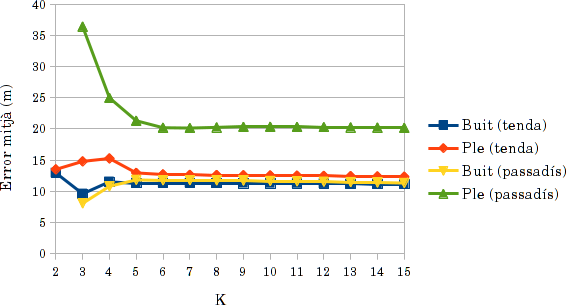
\includegraphics[width=8cm]{imatges/mmse_mitja.png}
\caption{Comparació gràfica de l'error per l'algorisme \textit{Probabilistic Minimum Mean Square Error} en passadissos (dalt) i botigues (abaix).}
\label{fig:grafic_mitja_MMSE}
\end{center}
\end{figure}

Pel que fa a la dispersió de les estimacions (figura \ref{fig:grafic_desviacio_MMSE}), la presència de persones augmenta la desviació mitjana en la gran majoria de casos. Només per valors de K petits els entorns sense usuaris mostren una dispersió menor, però cal tenir en compte les irregularitats abans mencionades en aquests casos. 

\begin{figure}[ht]
\begin{center}
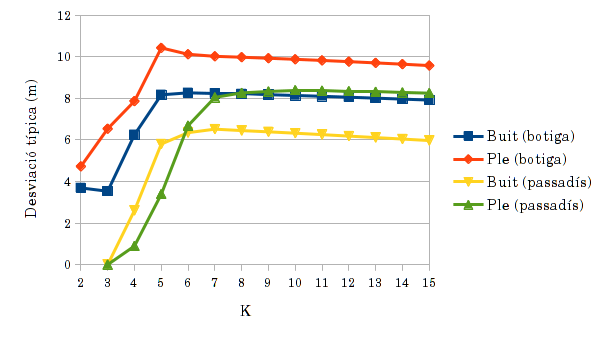
\includegraphics[width=8cm]{imatges/mmse_desviacio.png}
\caption{Comparació gràfica de l'error per l'algorisme \textit{Probabilistic Minimum Mean Square Error} en passadissos (dalt) i botigues (abaix).}
\label{fig:grafic_desviacio_MMSE}
\end{center}
\end{figure}
